%------------------------------------------------------------------------------
\chapter{Implementation details}
\label{ch:implementation_details}


\section{Application Overview}
\label{sec:application_overview}

Explain how to use the shaders and the commands


\section{\MentalRay Shading Approach}
\label{sec:mental_ray_shading_approach}

How mental ray shoots rays around and what is its paradigm.
Add pretty pictures of ray shooting.

\begin{figure}[htbp!]
\centering
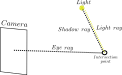
\includegraphics[width=0.8\textwidth]{img/mental_ray_model}
	\caption{\MentalRay simple ray casting example.}
	\label{fig:voxel_dataset_threaded}
\end{figure}

Equation~\ref{eq:rte_solution_paper} provides a radiance value for the next march increment, however we want to compute the value at the ray intersection with the volume, i.e. at the ray origin.
So we need to rewrite the equation as

\begin{equation}
\label{eq:rte_solution_paper}
\begin{split}
L(\lambda, \x, \omegam) &= e^{\sigma_t(\lambda, \x) \deltax} L(\lambda, x + \Delta\x, \omegam) +  \\
& (1 - e^{\sigma_t(\lambda, \x) \deltax} ) \frac{\sigma_a(\lambda, \x) L_e(\lxo) + \sigma_s(\lambda, \x) L_i(\lxo)}{\sigma_t(\lambda, \x)}.
\end{split}
\end{equation}

\section{Shaders Internals}
\label{sec:shaders_internals}

Talk about things like which parts are written in parallel code, instance support, shader internal memory, sparse data, how the software escalates, memory consumption, Maya integration, spectrum to rgb integration, maybe more details about units for black body radiation and everything that was not explained before

\begin{figure}[htbp!]
\centering
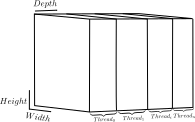
\includegraphics[width=0.8\textwidth]{img/voxel_thread_division}
	\caption{Voxel Dataset division of coefficients computation in threads.}
	\label{fig:voxel_dataset_threaded}
\end{figure}

\subsection{Fire Volume Shader}
\label{sec:fire_volume_shader}



\subsection{Fire Light Shader}
\label{sec:fire_light_shader}


\subsection{Voxel Dataset Shader}
\label{sec:voxel_dataset_shader}